\documentclass[a4paper, 12pt]{article}
\usepackage[utf8]{inputenc}
\usepackage[T1]{fontenc}
\usepackage{titlesec}
\usepackage{listings}
\usepackage{tikz}
\usetikzlibrary{shapes, arrows}

\tikzstyle{rect} = [rectangle, draw, minimum width=7em, minimum height=2em, rounded corners]
\tikzstyle{line} = [draw, -latex']

\lstset{basicstyle=\ttfamily, keepspaces=true}

\titleformat*{\section}{\Large\bfseries}

\title{\bf [PRI] Projekt pierwszy}
\author{Adrian Brodzik}

\begin{document}

\maketitle

\section*{Zadanie}
Napisz program, który wypisze linię znaków wejściowych zastępując każdy ciąg białych znaków pojedynczym znakiem ukośnika, zaś ewentualne każde wystąpienie ukośnika w linii zastąpi podwójnym ukośnikiem.
\\
\\
Dla danych wejściowych:\\
\lstinline{bfvrhowev h7u893  njio nvfrowe/vtgrw         vvv}
\\
\\
Poprawnym wynikiem jest:\\
\lstinline{bfvrhowev/h7u893/njio/nvfrowe//vtgrw/vvv}

\section*{Problem}
Opis problemu...

\section*{Rozwiązanie}
Opis rozwiązania...

\section*{Specyfikacja programu}
Użyte biblioteczki, funkcje, uzasadnienie...

\section*{Schemat działania}
\begin{center}
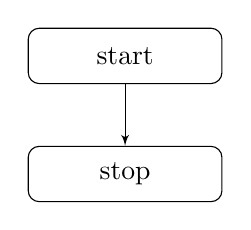
\begin{tikzpicture}[node distance = 1.5cm, auto]
\node [rect] (start) {start};
\node [rect, below of=start] (stop) {stop};
\path [line] (start) -- (stop);
\end{tikzpicture}
\end{center}

\section*{Testowanie}
Proces testowania i przykłady...

\section*{Podsumowanie}
Wnioski dotyczące projektu...

\end{document}
